I% Chapter Template

\chapter{Optimizations} % Main chapter title

\label{Optimizations} % Change X to a consecutive number; for referencing this chapter elsewhere, use \ref{ChapterX}

\lhead{\emph{Optimizations}} % Change X to a consecutive number; this is for the header on each page - perhaps a shortened title

%----------------------------------------------------------------------------------------
%	SECTION - Where does time go?
%----------------------------------------------------------------------------------------

\section{Where is time spent?}

%-----------------------------------
%	SUBSECTION 1
%-----------------------------------

\subsection{Arrays}
% array creation, copy
Most of the memory used in the vector data structure is composed of arrays. The three key operations used on these arrays: array creation, array update and array access. The arrays are used as immutable arrays, as such the update operations are only allowed when the array is initialized. This also implies that each time there is a modification on some part of an array, a new array must be created and all the old elements copied.  

% size of array argument
The size of the array will affect the performance of the vector. With larger blocks the access times will be reduced because the depth of the tree will decrease. But, on the other hand, increasing the size of the block will make slow down the update operations. This is a direct consequence of the need to copy the entire array for a single update.


%-----------------------------------
%	SUBSECTION 2
%-----------------------------------

\subsection{Computing indices}
\label{ComputingIndices}

Computing the indices in each node while traversing or modifying the vector is key in performance. This performances is gained by using low level binary computations on the indices in the case where the tree is balanced. And, using precomputed sizes in the case where the balance is relaxed.

%-----------------------------------
\paragraph{Radix}
% Explain how to compute them
Assuming that the tree is full, elements are fetched from the tree using radix search on the index. As each node has a branching of 32, the index can be split bitwise in blocks of 5 ($2^5 = 32$) and used to know the path that must be taken from the root down to the element. The indices at each level $L$ can be computed with $(index >> (5 \cdot L)) \& 31$. For example the index 526843 would be:
\[
 526843 = 00
   	 \underbracket[0.2pt][4pt]{00000}_{\text{0}}
   	 \underbracket[0.2pt][4pt]{00000}_{\text{0}}
  	 \underbracket[0.2pt][4pt]{10000}_{\text{16}}
 	 \underbracket[0.2pt][4pt]{00010}_{\text{2}}
	 \underbracket[0.2pt][4pt]{01111}_{\text{15}}
     \underbracket[0.2pt][4pt]{11011}_{\text{27}}
\]

\begin{lstlisting}[frame=single]
def getSubIndex(indexInTree: Int, level: Int): Int = 
  (index >> (5*level)) & 31
\end{lstlisting}

% how to generalise
This scheme can be generalised to any block size $m$ where $m=2^i$ for $0 < i \leq 31$. The formula would be $(index >> (m \cdot L)) \& ((1<<m)-1)$. It is also possible to generalise for other values of $m$ using the modulo, division and power operations. In that case the formula would become $(index / (m^L)) \% m$. This last generalisation is not used because it reduces sightly the performance and it complicates other index manipulations. 

\begin{figure}[h!]
  \centering
  \includegraphics[width=0.5\textwidth]{Figures/Radix_Balanced_index_example}
  \caption{Accessing element at index 526843 in a tree of depth 5. Empty nodes represent collapses subtrees.}
  \label{radix_balanced_index_example}
\end{figure}

%-----------------------------------
\paragraph{Relaxing the Radix}
% Explain how to compute them 
When the tree is relaxed it is not possible to know the sub-indices from index. That is why we keep the sizes array in the unbalanced nodes. This array keeps the accumulated sizes to make the computation of sub-indices as trivial as possible. The sub-index is the same as the first index in the sizes array where $index < sizes[subIndex]$. The simplest way to find this sub-index is by a linearly scanning the array. 

\begin{lstlisting}[frame=single]
def getSubIndex(sizes: Array[Int], indexInTree: Int): Int = {
  var is = 0
  while (sizes(is) <= indexInTree)
    is += 1
  is
}
\end{lstlisting}

% linear vs binary search
For small arrays (like blocks of size 32) this will take be faster than a binary search because it takes advantage of the cache lines. If we would consider using bigger block sizes it would be better to use a hybrid between binary and linear search.

% fallback to radix
To traverse the tree down to the leaf where the index is, the sub-indices are computed from the sizes as long as the tree node is unbalanced. If the node is balanced, then the more efficient radix based method is used from there to the leaf. To avoid the need of accessing and scanning an additional array in each level.


%-----------------------------------
%	SUBSECTION 3
%-----------------------------------

\subsection{Abstractions}
\label{sec:Abstractions}
When creating an implementation for a data structure it is always a good practice to have simple abstractions to simplify the code. This makes the code easier to read an reason about but it will complicate the execution of such a code. In this section we'll focus on how the actual implementation optimises out overheads that would be generated by functions and generic code abstractions.

% functions
\paragraph{Functions} When writing an algorithm we usually divide it into small self-contained subroutines and we try to factor out common the common ones. In practice this will add overhead for function invocations each time a function is used and break the locality of the code. To improve the performance we avoid as much as possible function call on simple operations. The code also avoids the creation of any higher order function to avoid additional object allocations. As such \texttt{while} loops are used rather than \texttt{for} loops.

%-----------------------------

\paragraph{Generalization}
A common way to reduce the amount of code that needs to be written when implementing common functionality is using generalization of code. But this comes with a computational cost for cases where a second implementation that takes into account the context of to simplify the operation. When considered beneficial the code is specialized by hand on the current context\footnote{This is specialisation on values not on types}. 

% generic code vs specialized code (specialized values, expanded loops)
The base mechanisms to specialize are: specialisation of a value, loops unrolling and arithmetic simplifications. Value specialization consist in explicitly identifying the value of some field and then using code specialized on that value. Loop unrolling (including recursions) consist in writing explicitly the code for each loop instead of the loop. This one is usually used on loops that are bounded by some value specialization. Once the first two specialisation are applied code can be simplified with arithmetic transformations. 

% example with simple expanded get operation (show expansion and specialisation)
Concretely, most of the value specialization is done on heights and indices on radix operations. The height are a bounded small range of numbers and therefore can be efficiently specialized with a \texttt{match}\footnote{All \texttt{match} expressions used in this specialization get compiled to \texttt{tableswitch} bytecode instruction. In some cases it would be beneficial to have  \texttt{tableswitch} with fallthrough, but the there is currently no Scala construct that compiles to that.} expression. On ranges of indices that are on trees of the same size specialization is done using nested \texttt{if/else} expressions. It is also possible to specialize of the first and last index, the first index (the 0 index) gains much from specialization because of arithmetic cancelation of many terms. As an example here is a version of the radix \texttt{apply}. 

\begin{lstlisting}[frame=single]
def apply(index: Int): A = {
    vectorDepth match {
      case 1 => 
        vectorRoot(indexInNode & 31)
      case 2 => 
        val node1 = vectorRoot((indexInNode>>5) & 31)
        node1(indexInNode & 31)
      case 3 => 
        val node2 = vectorRoot((indexInNode>>10) & 31)
        val node1 = node2((indexInNode>>5) & 31)
        node1(indexInNode & 31)
      case 4 =>
        ...
    }
  }
\end{lstlisting}

Where the \texttt{vectorDepth} is specialized, then the recursion is rolled and finally a \texttt{>>} is removed on each branch of the \texttt{match}. Taking this one setup further with the \texttt{head} method that is usually implemented as \texttt{apply(0)}, using the same specialization the code becomes:

\begin{lstlisting}[frame=single]
def head(): A = {
    vectorDepth match {
      case 1 => vectorRoot(0)
      case 2 => vectorRoot(0)(0)
      case 3 => vectorRoot(0)(0)(0)
      ...
    }
  }
\end{lstlisting}
Removing the need for any additional arithmetic operation. The actual implementation differs from this one because it also aims to take advantage of displays (see \ref{sec:Displays}) to avoid starting from the root in some cases.

In relaxed radix operation the loop unrolling is usually avoided because in those methods the amount of nodes traversed can't be known in advance. But will invoke specialized versions of the code as soon as it finds a node on which it is possible. For a perfectly balanced RRB-Tree that node is to root, and hence the performance for such vectors is similar to the one for an RB-Tree.

%----------------------------------------------------------------------------------------
%	SECTION - Displays
%----------------------------------------------------------------------------------------
\clearpage
\section{Displays}
\label{sec:Displays}
% describe display fields in vector object
As base for optimizations, the vector object keeps a set of fields to track one branch of the tree. They are named with using the level number from 0 up to the maximum possible level. In the case of blocks of size 32 the maximum level used is 5\footnote{As in practice, only the 30 bits of the index are used.}, they are allocated by default and nulled if the tree if shallower. The highest non null display is and replaces the root field. All displays bellow the root are never null. This implies that the vector will always be focused on some branch.

\begin{figure}[h!]
  \centering
  \includegraphics[width=0.8\textwidth]{Figures/Displays}
  \label{Displays}
  \caption{Displays}
\end{figure}

% describe the focus field
To know on which branch the vector is focused there is also a \texttt{focus} field with an index. This index is the index of any element in the current \texttt{display0}. This index represents the radix indexing scheme of node sub-indices described in \ref{ComputingIndices}. 

% immutability of displays
To follow the simple implementations scheme of immutable objects in concurrent contexts, the focus is also immutable. Therefore each vector object will have a single focused branch during its existence\footnote{The display focus may change during the initialisation of the object as optimisation of some methods}. Each method that creates a new vector must decide which focus to set. 

%-----------------------------------
%	SUBSECTION As cache
%-----------------------------------

\subsection{As cache}
% used to access some elements directly from the smaller subtrees (XOR)
One of the uses of the displays is as a cached branch. If the same leaf node is used in the following operation, there is no need for vertical tree traversal which is key to amortize operation to constant time. In the case another branch in needed, then it can be fetched from the lowest common node of the two branches. 

% xor
To know the which is the level of the lowest common node in a vector of block size $2^m$ (for some consistent $m$), only the \texttt{focus} index and the index being fetched are needed. The operation $index XOR focus$ will return a number is bounded to the maximum number of elements in a tree of that level. The actual level can be extracted with some if statements. This operation bounded by the same number of operations that will be needed to traverse the tree back down through the new branch.

\begin{lstlisting}[frame=single]
def getLowestCommonLevel(index: Int, focus: Int): Int = {
  val xor = index ^ focus
  if (xor < 32 /*(1<<5)*/ ) 0
  else if (xor < 1024 /*(1<<10)*/ ) 1
  else if (xor < 32768 /*(1<<15)*/ ) 2
  ...
  else 5
}
\end{lstlisting}

% keeping relevant branch for next operations
When deciding which will be the focused branch of a new vector two heuristics are used for this: If there was an update operation on some branch where that operations could be used again, that branch is used as focus. If the first one cant be applied, the display is set to the first element as this helps key collection operations such as \texttt{iterator}.

%-----------------------------------
%	SUBSECTION  For transient states
%-----------------------------------

\subsection{For transient states}
\label{sec:DisplaysTransient}
% operation: append, prepend, update
Transient states is the key optimisation to get append, prepend and update to amortized constant time. It consists in decoupling the tree by creating an equivalent tree that does not contain the edges on the current focused branch. The information missing in the edges of the tree is represented and can be reconstructed from the displays. In the current version of the collections vector \cite{scalaVector211} this state is identified by the \texttt{dirty} flag.

\begin{figure}[h!]
  \centering
  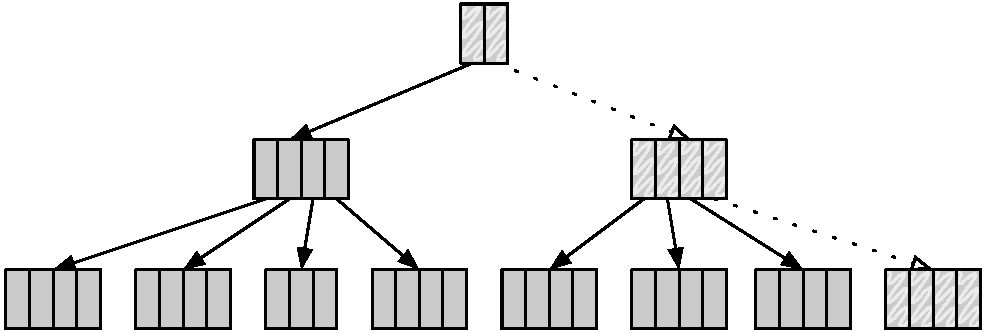
\includegraphics[width=0.8\textwidth]{Figures/Transient_state}
  \label{Transient_state}
  \caption{Transient Tree with current focus displays marked in white and striped nulled edges.}
\end{figure}

% transient states are used to amortized operations
Without transient states when some update is done on a leaf, all the branch must be updated. On the other hand, if the state is transient, it is possible to update only the subtree affected by the change. In the case of updates on the same leaf, only the leaf must be updated. When appending or prepending, $\frac{31}{32}$ operations must only update the leaf, then $\frac{31}{1024}$ need to update two levels of the tree and so on. These operations will thus be amortized to constant ($\sum_{k=1}^{\infty} \frac{k*31}{32^k} = \frac{32}{31}$ block updates per operation) time if they are executed in succession.

% normailization
There is a cost associated to the transformation from canonical to transient state and back. This cost is equivalent to one update of the focused branch. The transient state operations only start gaining performance on the canonical ones after 3 consecutive operations. With 2 consecutive operations they are matched and with 1 there is a loss of performance.

%-----------------------------------
%	SUBSECTION  Relaxing the Displays
%-----------------------------------

\subsection{Relaxing the Displays}
% describe fundamental difference in the focus (focused on balanced subtree)
When relaxing the tree balance it is also necessary to relax the displays. This is mainly due to the loss of a simple way to compute the lowest common node on unbalanced trees. Computing the node requires now the additional sizes information located in each unbalanced node. As such it is necessary to access the nodes to be able to compute the lowest common node, and there is a loss in performance due to increased memory accesses.  

% describe focus start, focus end and focus (focus relaxed)
To still take advantage of efficient operations on balanced trees, the display is relaxed to be focused on a branch of some balanced subtree\footnote{A fully balanced tree will be itself the balanced subtree, as such it will always use the more performant operations.}. To keep track of this subtree there are three additional fields: \texttt{focusStart} that represents start index of the current focused subtree, \texttt{focusEnd} that represents the end index of the subtree and \texttt{focusDepth} that sets  height of the focused subtree\footnote{As an optimisation, the \texttt{focus} field is split into the part corresponding to the subtree and the part that represents the indices of the displays that are unbalanced.}. The operations that can take advantage of the the efficient display operations will check if the index is in the subtree index range and invoke the efficient operation. If not, it will invoke the relaxed version of the operation, that starts from the root of the tree.

% describe how fetching elements change
For example, the code for \texttt{getElement} would become:
\begin{lstlisting}[frame=single]
def getElement(index: Int): A = {
  if (focusStart <= index && index < focusEnd) 
    getElementFromDisplay(index - focusStart)
  else if (0 <= index && index < endIndex) 
    getElementFromRoot(index)    
  else 
    throw new IndexOutOfBoundsException(index)
}
\end{lstlisting}

This \texttt{getElement} on the unbalanced subtrees of figure \ref{Balanced_subtrees}  would use the \texttt{getElementFromDisplay} to fetch elements in \texttt{display0} directly from it and fetch elements from nodes (1.1) and (1.2) starting from \texttt{display1}. The rest is fetched from the root using \texttt{getElementFromRoot}.

\begin{figure}[h!]
  \centering
  \includegraphics[width=\textwidth]{Figures/Balanced_subtrees}
  \caption{Relaxed Radix Balanced Tree with a focus on a balanced subtree rooted of \texttt{display1}. Light grey boxes represent unbalanced nodes sizes.}
  \label{Balanced_subtrees}
\end{figure}

%-----------------------------------
%	SUBSECTION  Vector Canonicalization
%-----------------------------------

\subsection{Vector Canonicalization}
\label{VectorCanonicalization}
% State can mutate from transient to canonical exactly once (similar to lazy evaluation)
% State mutation is not visible from outside
% If more performance is requires it is possible to write transient state operations directly to transient state
As started in section \ref{sec:DisplaysTransient} vectors have two representation: canonical and transient. The transient state aims to improve performance of some operations by amortising costs. But, the transient state is not ideal for performance of other operations. For example an \texttt{apply} operation on an unbalanced vector may lack the sizes information it requires to access certain indices. And an iterator relies on a canonical tree for performance. It is always possible to implement those operations on transient states, but they would involve additional overhead on each call and duplication of code.

The solution is to convert the transient representation to a canonical one when an operation that requires it is called on an instance of the immutable vector. The mutation of the vector is not visible from the outside and only happens at most once. This transformation only affects the nodes that are on the display, it copies each one (except the leaf) and links the trees. If the node is unbalanced, the size of the subtree in focus is inserted. This transformation could be seen as a lazy initialization of the current branch.

% Explain append/prepend
Vector objects can only be in transient state if they where created that way. For example, the \texttt{append}/\texttt{prepend} operation will create a new object that is in transient state and focused on the last/first branch. If the source object was not focusing the last branch, then it is canonicalized (if needed) before change of branch operation. Vectors depth 1 are special cases, they are always in canonical form and their operations are equivalent to those in transient form.

Figure \ref{StatesGraphSimple} shows the different states and the effects of the \texttt{append} and \texttt{apply} operations on them. Figure \ref{StatesGraphComplete} shows the same for all operations. Note that the mutation of \texttt{this} object only happened from transient to canonical and that the only way to get to transient is with a creation of a new vector object.

\begin{figure}[h!]
  \centering
  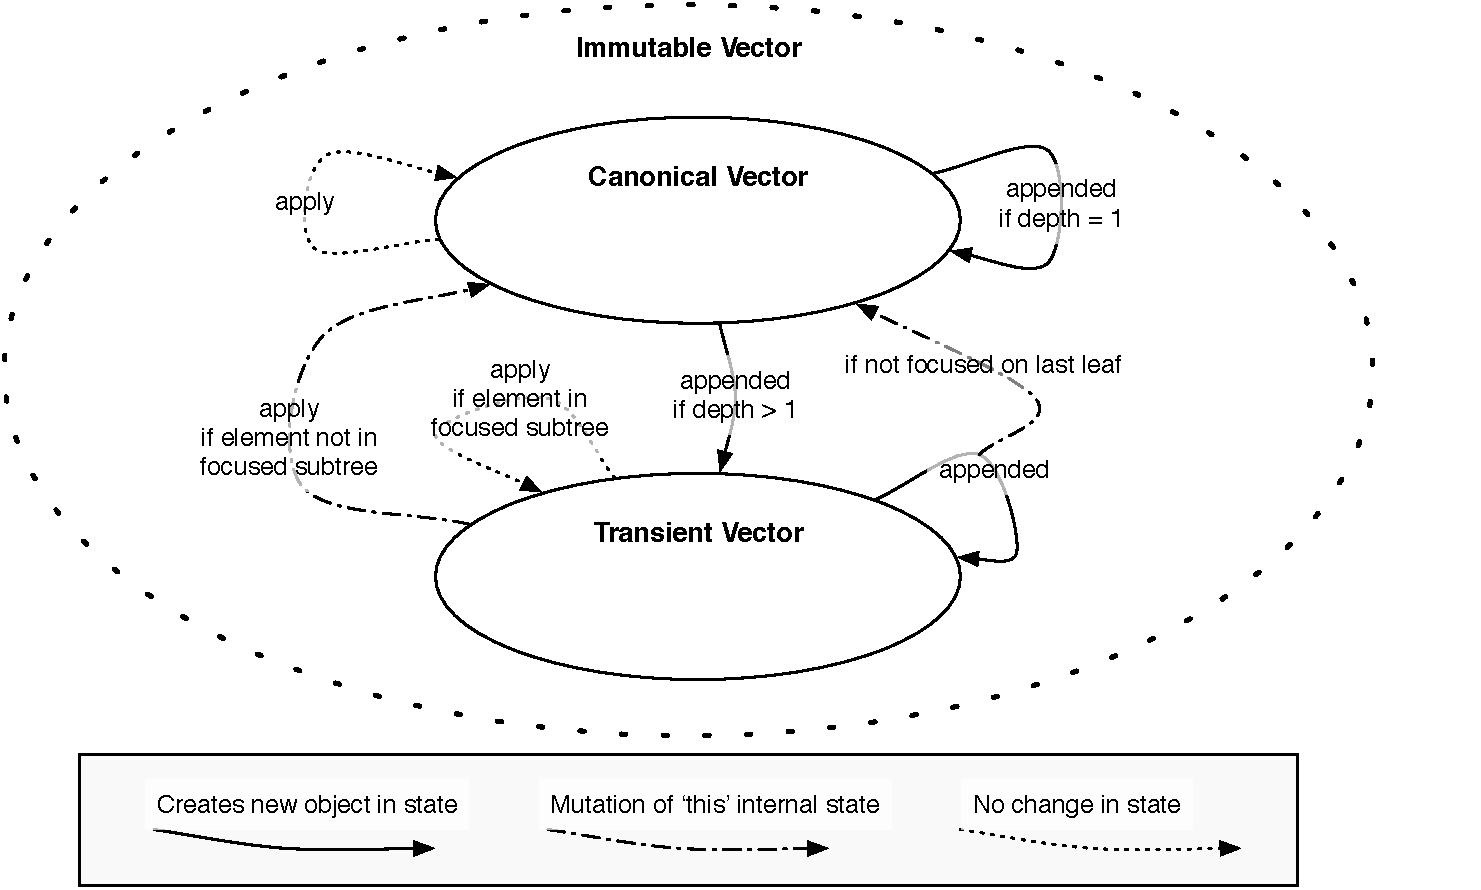
\includegraphics[width=0.8\textwidth]{Figures/StatesGraphSimple}
  \caption{}
  \label{StatesGraphSimple}
\end{figure}


\begin{figure}[h!]
  \centering
  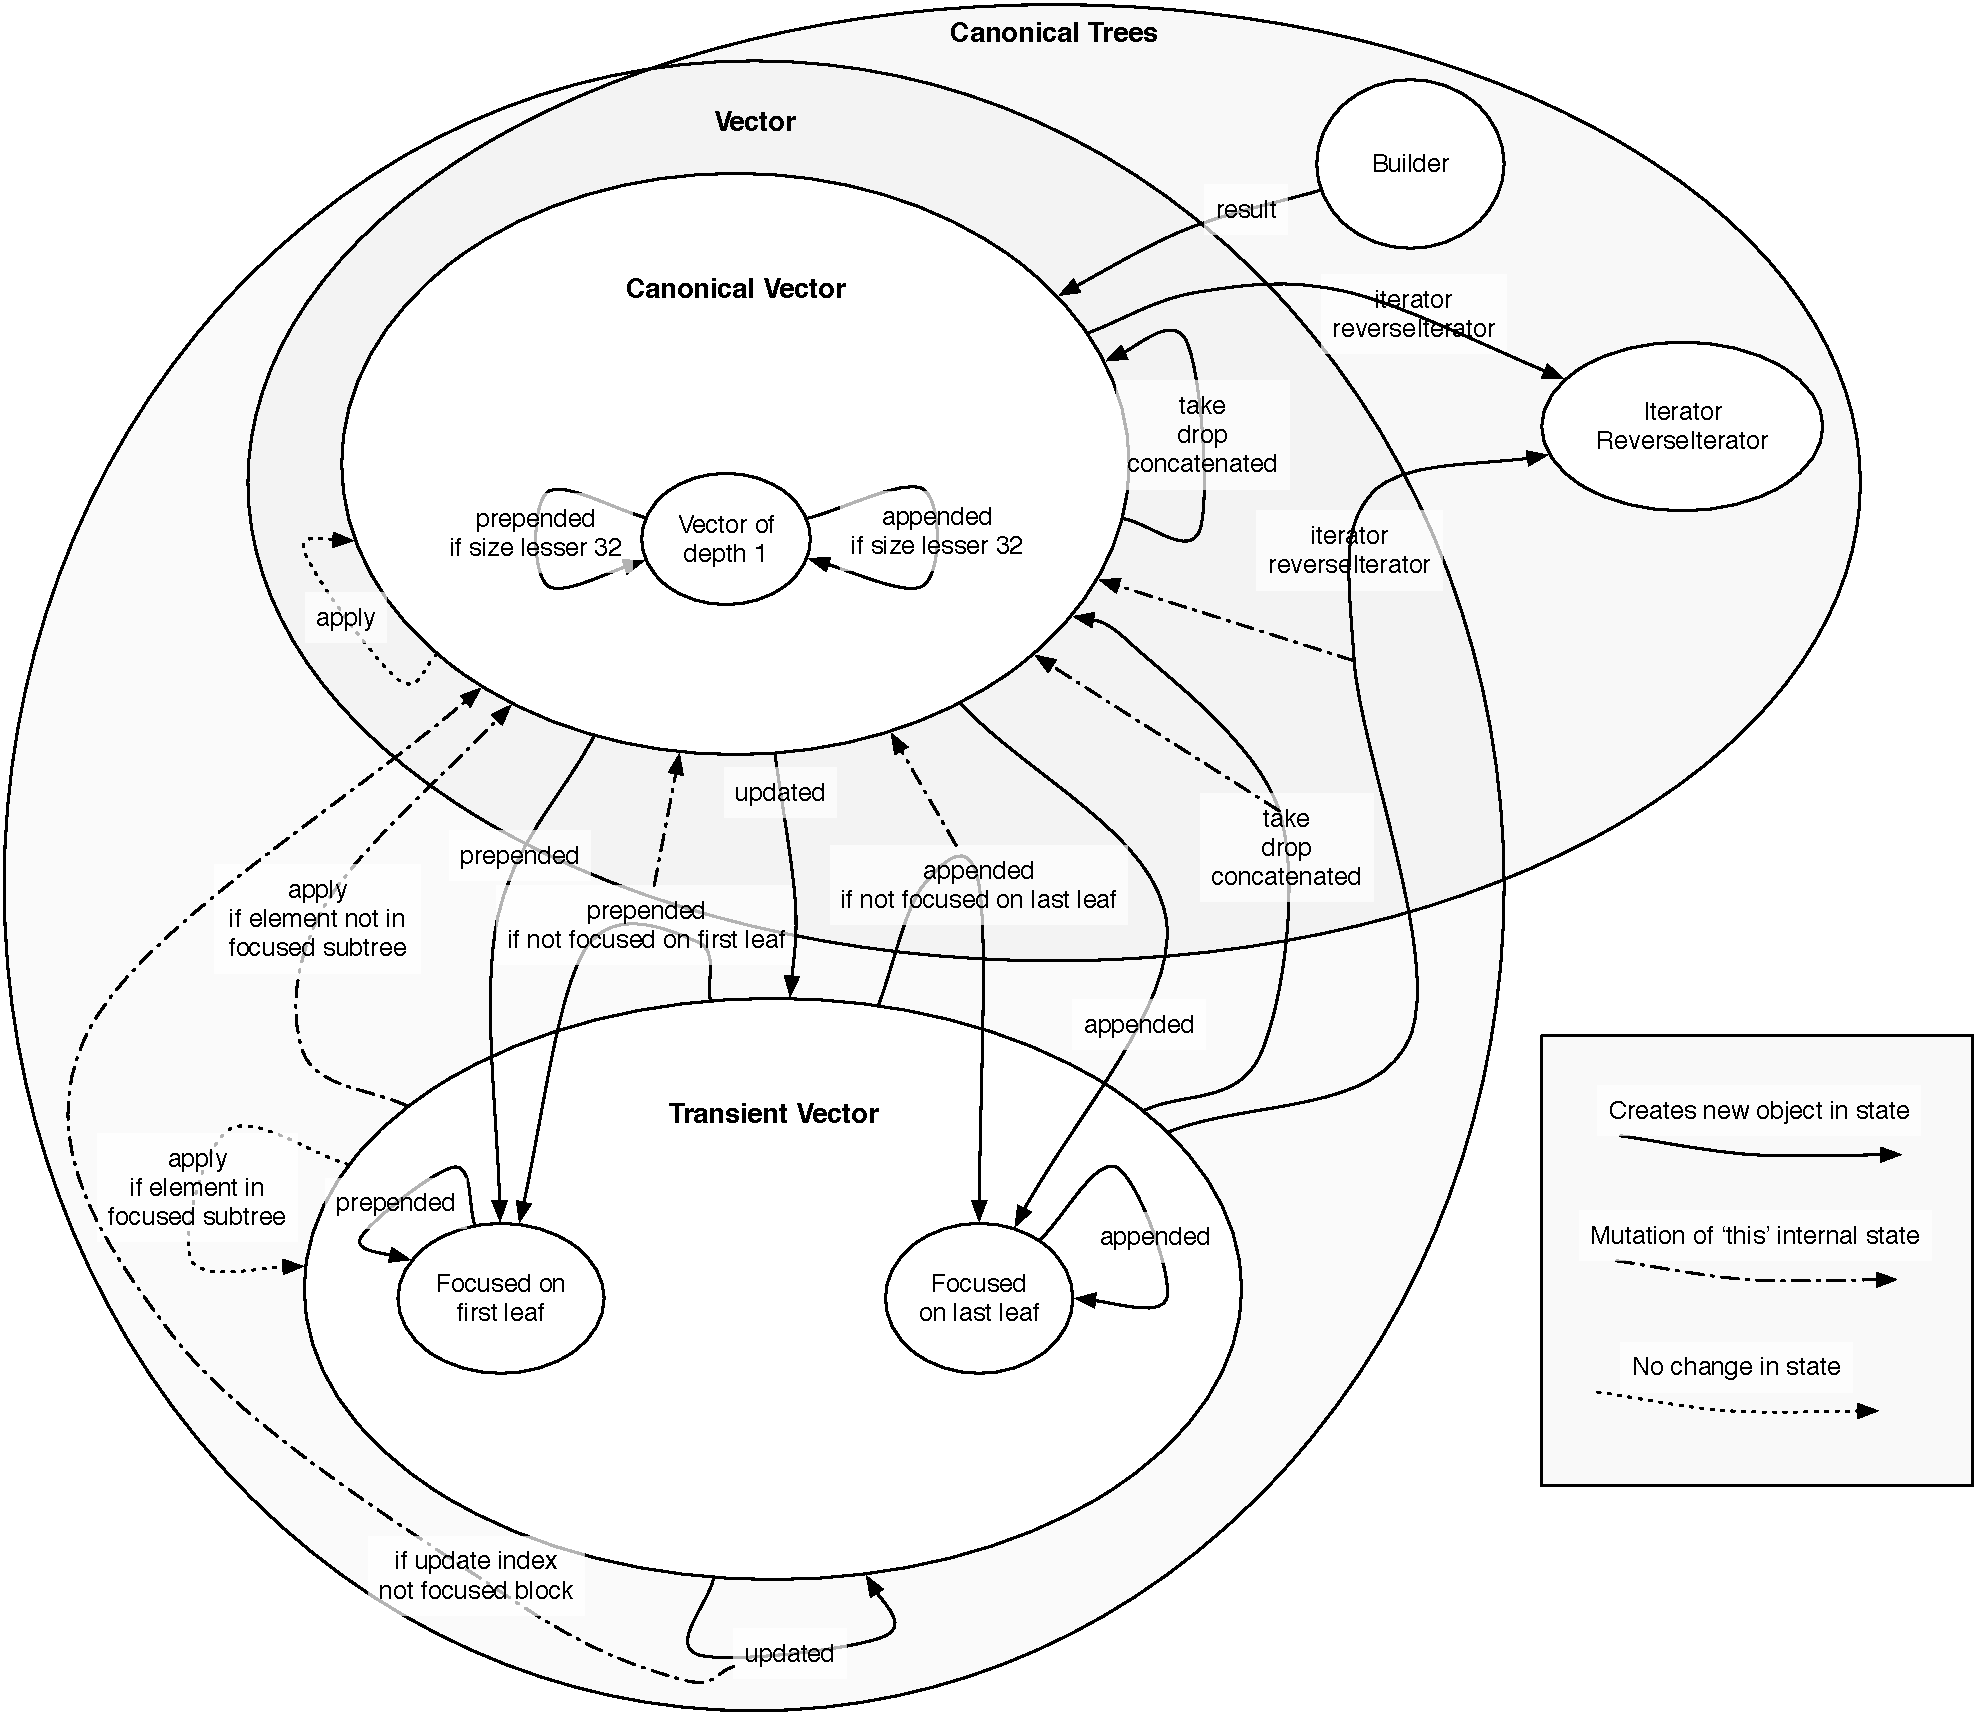
\includegraphics[width=\textwidth]{Figures/StatesGraph}
  \caption{}
  \label{StatesGraphComplete}
\end{figure}

%----------------------------------------------------------------------------------------
%	SECTION - Builder
%----------------------------------------------------------------------------------------
\clearpage
\section{Builder}
% use of mutable tree 
% avoid creation unnecessary arrays
A vector builder is a special wrapper for a RB-Tree that has an efficient \texttt{append} operation. It is implemented using encapsulated mutable arrays during the building of the vector and then frozen on the creation of the result. Any array that the builder can still mutate is cloned and possibly truncated to generate the RB-tree of the vector. 

The benefits of the mutable \texttt{append} operation of the builder over \texttt{appended} operation of the vector are on the reduced amount of memory allocations needed in the process of appending. There is no need to allocate a new \texttt{Vector} object each time an element is appended. Even more important is that there is no need to create a new array in each charge on a node, nodes are allocated one and field as needed. 

%-----------------------------------
\paragraph{Relaxing the Builder}
% same base implementation for +=
% addition of accumulator for  ++= 
Most of the operations implemented in the collections framework that use builder usually create the new collection by appending one element at a time. To retain the performance of all existing operation that use builders the implementation builder append does not change. Therefore the tree where elements are appended is always perfectly balanced.
 
 To add performance when concatenating a \texttt{Vector} to a builder a new field is added to retain a vector that will be lazily concatenated to the result. This vector is the accumulation \texttt{acc} of every all elements (vectors) that where added before (and including) the last concatenation and elements in the current tree been build. All elements added after the last concatenation are added to the main the mutable tree of the builder.


%----------------------------------------------------------------------------------------
%	SECTION - Iterator
%----------------------------------------------------------------------------------------
\clearpage
\section{Iterator}
% efficient tree traversal vs iteration by index
% avoid re-traversing vertically the tree from the root
The default implementation for iterator in \texttt{IndexedSeq} is by iterating on the indices and for each one use the \texttt{apply} method on it. This is not optimal because it requires traversing the tree down from the root each time an element is accessed. The traversal of the vector using this would have a computational complexity of $O(n \cdot log_{32}(n))$.

To improve performance of the iteration on vector a normal tree traversal of the underlying RB-Tree amortizes the computational complexity to $O(n)$. The iterator can use the display optimization to keep track of the current branch and move to the next branches efficiently using the radix index scheme. In this case the display is allowed to mutate. The current implementation of vector is implemented this way\footnote{The current \texttt{reverseIterator} is still using traversal by index.}. 

%-----------------------------------
\paragraph{Relaxing the Iterator}
% same implementation within a balanced subtree
% refocus from root to iterate between balanced subtrees
To keep the performance advantages of the tree traversal on balanced RRB-trees, iteration is done the same on every balanced subtree. When the end of a balanced subtree is reached the first element of the next balanced subtree is focused and the traversal continues efficiently from there. If the tree is not too unbalanced the traversal will tend to be $O(n)$. But if the tree is extremely unbalanced it will tend to fall back on $O(n \cdot log_{32}(n))$, where the additional $log_{32}(n)$ comes from the changes of balanced subtrees. Even in this bad last case the performance is better than the traversal by index because each leaf is a balanced subtree, on which efficient traversal is used. The RRB-Vector implements both \texttt{iterator} and \texttt{reverseIterator} this way.






